% LaTeX snippets for all generated figures.  The writing-agent embeds
% these inline into main.tex rather than \input{}-ing this file.

\begin{figure}[ht]
  \centering
  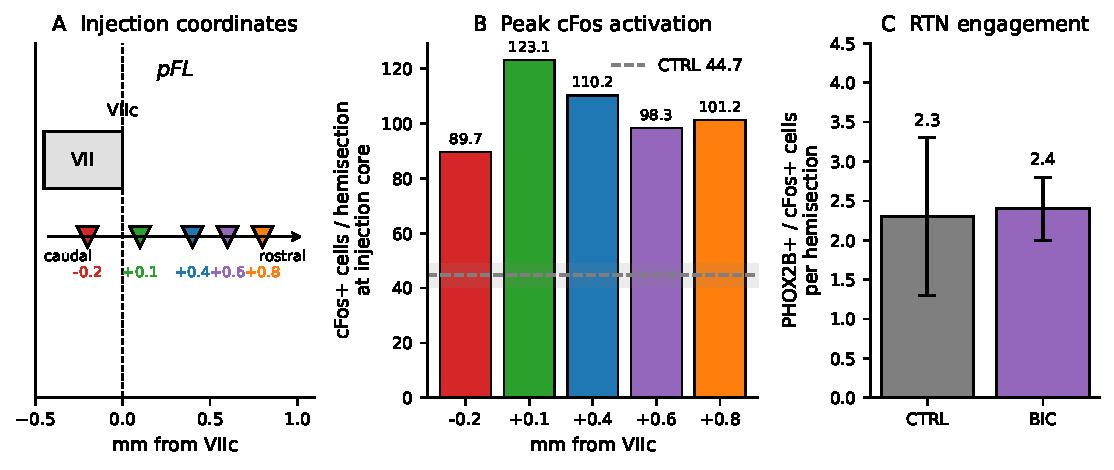
\includegraphics[width=0.95\linewidth]{figures/fig1_schematic_cfos.pdf}
  \caption{\textbf{Experimental design and anatomical verification.}
  \textbf{A} Schematic of the five bilateral rostrocaudal coordinates
  (-0.2, +0.1, +0.4, +0.6, +0.8\,mm from the caudal tip of the facial nucleus,
  VIIc) sampled by pressure injection of bicuculline in the parafacial lateral
  (pFL) region. \textbf{B} Peak cFos$^+$ cell counts per hemisection at the
  core of each bicuculline injection (bars) vs.\ the HEPES vehicle control
  (grey dashed line, 44.7$\pm$4.0). \textbf{C} Counts of double-labelled
  PHOX2B$^+$/cFos$^+$ cells per hemisection are indistinguishable between
  CTRL and bicuculline, indicating that the retrotrapezoid nucleus is not
  recruited by pFL disinhibition.}
  \label{fig:fig1}
\end{figure}

\begin{figure}[ht]
  \centering
  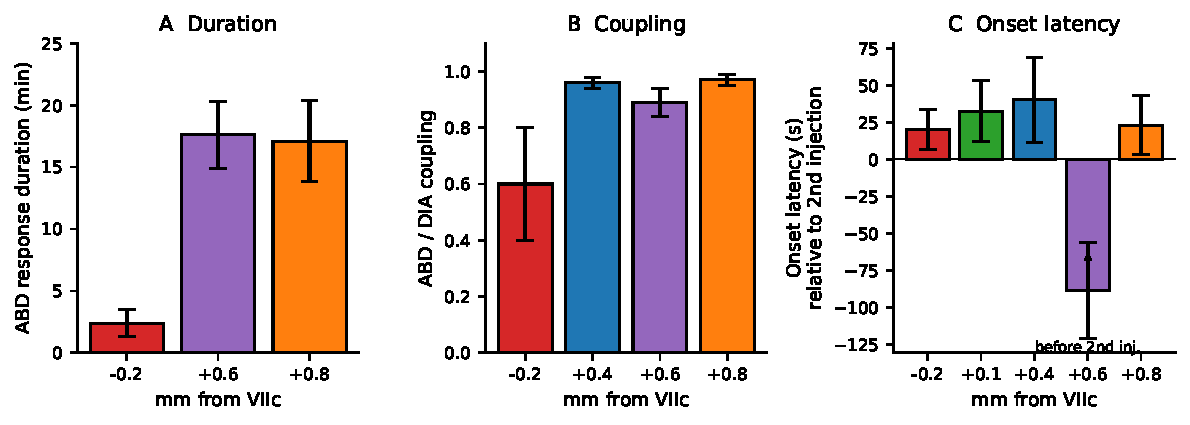
\includegraphics[width=0.95\linewidth]{figures/fig2_abd_temporal.pdf}
  \caption{\textbf{Temporal characteristics of the abdominal (ABD) EMG
  response to bicuculline.} \textbf{A} ABD response duration is markedly
  longer at the two most rostral sites (+0.6\,mm = 17.6$\pm$2.7\,min;
  +0.8\,mm = 17.1$\pm$3.3\,min) than at the caudal site (-0.2\,mm =
  2.4$\pm$1.1\,min; ANOVA $p=0.043$, $\eta^2=0.41$). \textbf{B} Peak
  ABD/DIA coupling. \textbf{C} Onset latency relative to the second
  bicuculline injection: at +0.6\,mm the response begins on average
  88.7$\pm$32.3\,s \emph{before} the second injection.}
  \label{fig:fig2}
\end{figure}

\begin{figure}[ht]
  \centering
  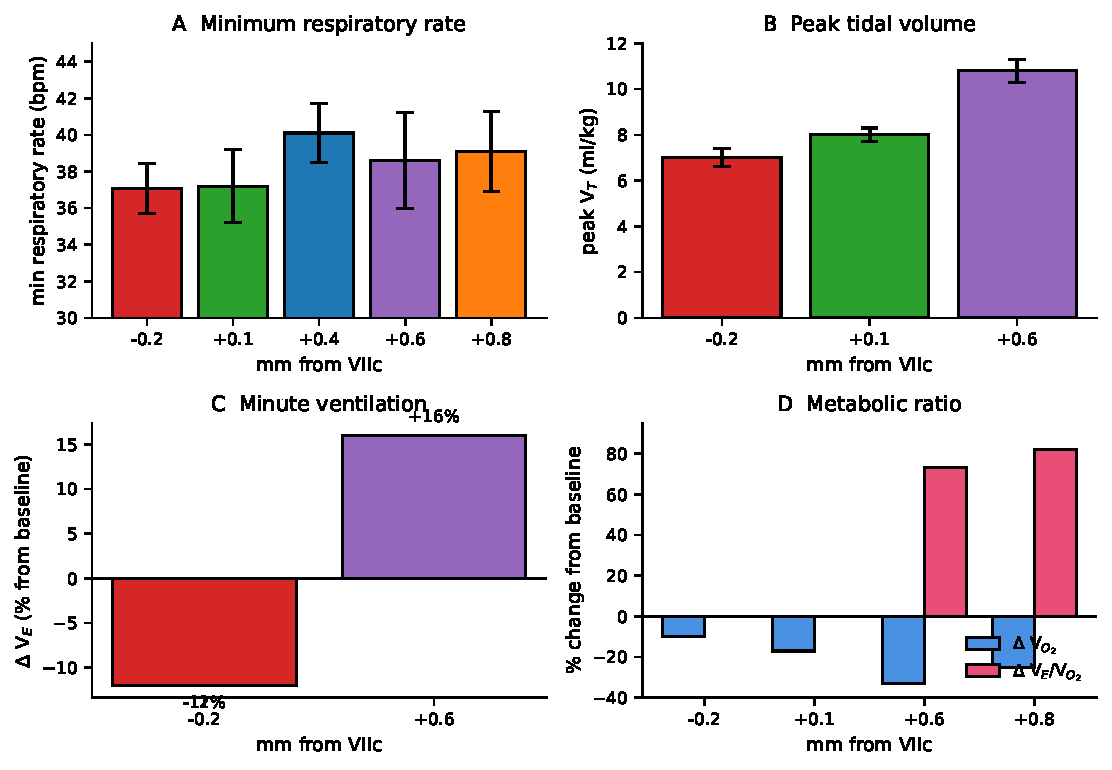
\includegraphics[width=0.95\linewidth]{figures/fig3_respiratory_metabolic.pdf}
  \caption{\textbf{Respiratory and metabolic effects scale with rostrocaudal
  coordinate.} \textbf{A} Minimum respiratory frequency reached in each
  group. \textbf{B} Peak tidal volume; the largest peak V$_T$ is at +0.6\,mm
  (10.8$\pm$0.5\,ml\,kg$^{-1}$, a 29\% increase from baseline). \textbf{C}
  Percent change in minute ventilation: V$_E$ decreases by 12\% at -0.2\,mm
  but rises by 16\% at +0.6\,mm. \textbf{D} Percent change in O$_2$
  consumption (blue) and in the V$_E$/V$_{O_2}$ ratio (red). V$_{O_2}$
  drops by 33\% at +0.6\,mm and 25\% at +0.8\,mm; V$_E$/V$_{O_2}$ rises by
  73--82\% only at rostral sites.}
  \label{fig:fig3}
\end{figure}

\begin{figure}[ht]
  \centering
  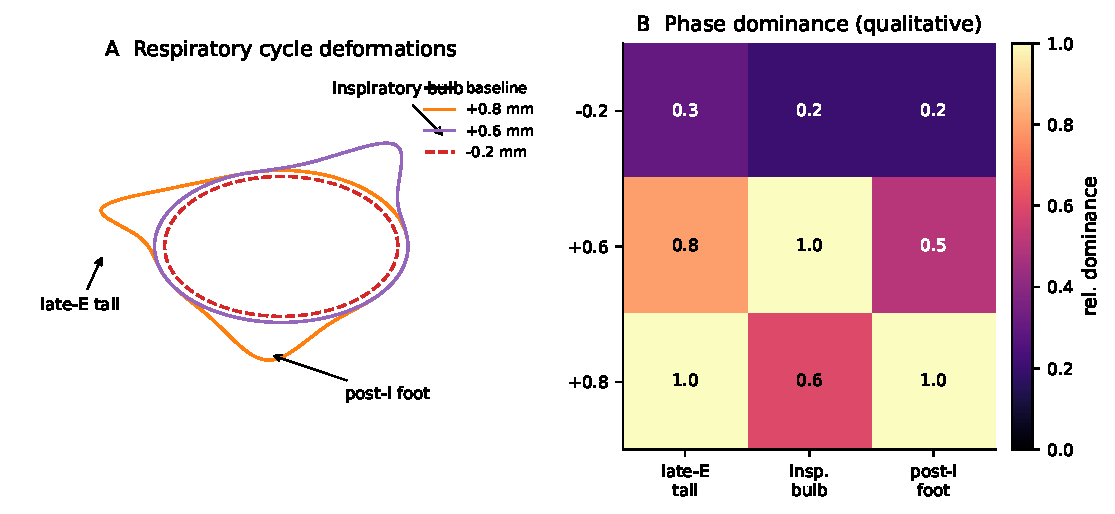
\includegraphics[width=0.95\linewidth]{figures/fig4_3d_trajectory.pdf}
  \caption{\textbf{3D respiratory trajectory analysis dissociates +0.6\,mm
  and +0.8\,mm responses.} \textbf{A} Schematic cycle in the
  airflow$\times$$\int$DIA$\times$$\int$ABD space. Baseline loop (black),
  compared with three injection-site signatures. +0.6\,mm produces the
  largest inspiratory ``bulb'', whereas +0.8\,mm produces the most extended
  late-expiratory ``tail'' and the largest post-inspiratory ``foot''.
  \textbf{B} Qualitative dominance of each cycle phase by injection group,
  summarising the statistical dissociations quantified in the Results.}
  \label{fig:fig4}
\end{figure}

\begin{figure}[ht]
  \centering
  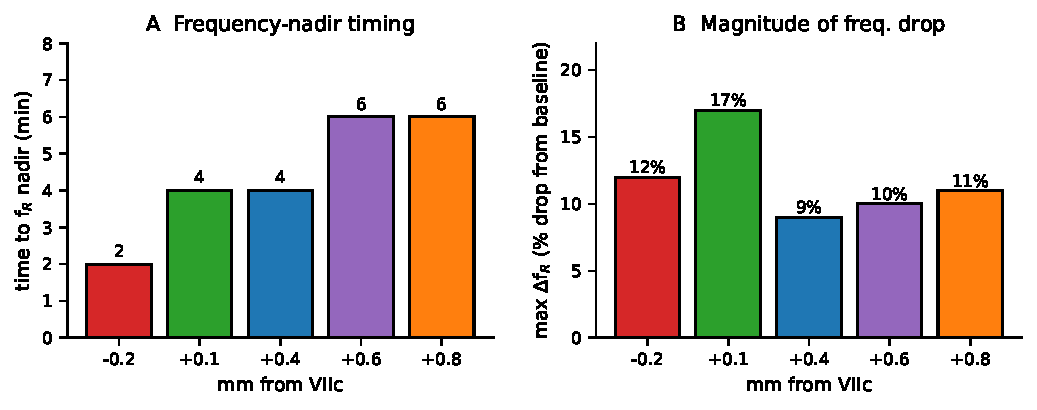
\includegraphics[width=0.85\linewidth]{figures/fig5_nadir_timing.pdf}
  \caption{\textbf{Rostrocaudal gradient in the timing of the frequency
  response.} \textbf{A} Time to minimum respiratory rate after injection
  increases from 2\,min at the most caudal site to 6\,min at the two most
  rostral sites. \textbf{B} Magnitude of the frequency drop (\% of baseline).}
  \label{fig:fig5}
\end{figure}
